\documentclass[a4paper,man,floatsintext,longtable,noextraspace,10pt]{apa6}

\usepackage[english]{babel}
\usepackage[utf8x]{inputenc}
\usepackage{amsmath}
\usepackage{graphicx}
\usepackage[colorinlistoftodos]{todonotes}
\usepackage{hyperref}

\usepackage{booktabs}
\usepackage{longtable}
\usepackage{array}
\usepackage{multirow}
\usepackage{wrapfig}
\usepackage{float}
\usepackage{colortbl}
\usepackage{pdflscape}
\usepackage{tabu}
\usepackage{threeparttable}
\usepackage{threeparttablex}
\usepackage[normalem]{ulem}
\usepackage{makecell}
\usepackage{xcolor}
% make captions italic

% number lines
% \usepackage{lineno}
% \linenumbers
            
% definitions for citeproc citations
\NewDocumentCommand\citeproctext{}{}
\NewDocumentCommand\citeproc{mm}{%
\begingroup\def\citeproctext{#2}\cite{#1}\endgroup}
\makeatletter
% allow citations to break across lines
\let\@cite@ofmt\@firstofone
% avoid brackets around text for \cite:
\def\@biblabel#1{}
\def\@cite#1#2{{#1\if@tempswa , #2\fi}}
\makeatother
\newlength{\cslhangindent}
\setlength{\cslhangindent}{1.5em}
\newlength{\csllabelwidth}
\setlength{\csllabelwidth}{3em}
\newenvironment{CSLReferences}[2] % #1 hanging-indent, #2 entry-spacing
{\begin{list}{}{%
  \setlength{\itemindent}{0pt}
  \setlength{\leftmargin}{0pt}
  \setlength{\parsep}{0pt}
  % turn on hanging indent if param 1 is 1
  \ifodd #1
  \setlength{\leftmargin}{\cslhangindent}
  \setlength{\itemindent}{-1\cslhangindent}
  \fi
  % set entry spacing
  \setlength{\itemsep}{#2\baselineskip}}}
{\end{list}}
\usepackage{calc}
\newcommand{\CSLBlock}[1]{\hfill\break\parbox[t]{\linewidth}{\strut\ignorespaces#1\strut}}
\newcommand{\CSLLeftMargin}[1]{\parbox[t]{\csllabelwidth}{\strut#1\strut}}
\newcommand{\CSLRightInline}[1]{\parbox[t]{\linewidth - \csllabelwidth}{\strut#1\strut}}
\newcommand{\CSLIndent}[1]{\hspace{\cslhangindent}#1}

% tightlist
\providecommand{\tightlist}{%
  \setlength{\itemsep}{0pt}\setlength{\parskip}{0pt}}

\shorttitle{}

% flow chart
\usepackage{tikz}
\usetikzlibrary{shapes.geometric, arrows, positioning, calc, shapes.multipart}

% Custom styles for the flowchart
\tikzstyle{datasource} = [rectangle, rounded corners, minimum width=2.5cm, minimum height=1cm,text centered, draw=blue!60, fill=blue!5]
\tikzstyle{process} = [rectangle, minimum width=3cm, minimum height=1cm, text centered, draw=green!60, fill=green!5]
\tikzstyle{decision} = [diamond, minimum width=3cm, minimum height=1cm, text centered, draw=red!60, fill=red!5]
\tikzstyle{arrow} = [thick,->,>=stealth]
\tikzstyle{output} = [rectangle, rounded corners, minimum width=3cm, minimum height=1cm, text centered, draw=purple!60, fill=purple!5]

\setlength\parindent{1.27cm}

\begin{document}
\thispagestyle{otherpage}

%\maketitle

% Change \title, \date, remove \author:
\begin{large}
\textbf{Replication: Hybrid Open Access in Transformative Agreements}
\end{large}

% Add below \maketitle:
\newcommand{\orcid}{%
  \begingroup\normalfont
  
\includegraphics[height=0.9em]{orcid_logo}% removed .png extension
  \endgroup
}

Najko Jahn\textsuperscript{1}\textsuperscript{*} 
(\orcid{} \href{https://orcid.org/0000-0001-5105-1463}{\color{black}{0000-0001-5105-1463}})

\textsuperscript{1} Göttingen State and University Library, University of Göttingen, Germany. \\

\textsuperscript{*} Correspondence: \href{mailto:najko.jahn@sub.uni-goettingen.de}{\color{black}{najko.jahn@sub.uni-goettingen.de}} 

\section*{Abstract}
{}
{\textbf{Keywords}: hybrid open access, transformative agreements, scholarly publishing, big deals, bibliometrics}

\newpage

% QSS wants numbered sections
\setcounter{secnumdepth}{2}

\section{Introduction}\label{introduction}

Transformative agreements are a much-discussed library licensing model
to transition subscription-based journal publishing to full open access.
While these agreements can vary substantially, they mainly target hybrid
journal portfolios, enabling researchers from participating institutions
to publish open access in them while also providing reading access to
the entire portfolio. Responding to experiences with the subscription
model, library consortia and funders have begun to coordinate the
standardisation of negotiation, administration, and evaluation practices
for these agreements. Simultaneously, efforts to improve transparency
through open data about contracts and payments are ongoing. However,
this information remains only partially available through bibliometric
databases, limiting large-scale studies about the impact of
transformative agreements on the transition of hybrid journals to full
open access. This study compares findings from hoaddata, an openly
available, continuously updated dataset on hybrid open access, built on
open data from Crossref, OpenAlex and the cOAlition S Journal Checker
Tool, with the established bibliometric databases Web of Science and
Scopus. The purpose of this comparison is not only to evaluate the
suitability of open metadata for measuring hybrid open access but also
to inform bibliometric research and practice by highlighting the
strengths and weaknesses of each data source.

Since the initial proposal to further develop hybrid open access as a
means to cost-effectively repurpose subscription spending toward open
access (Schimmer et al., 2015), transformative agreements have led to
considerable academic debate. While standardisation activities,
particularly through the OA2020 and ESAC (Efficiency and Standards for
Article Charges) initiatives, have led to improved workflows between
library consortia and publishers, as well as increased open access
publishing (Campbell et al., 2022; Geschuhn \& Stone, 2017), the initial
focus on a few large publishers by national consortia from high-income
countries has drawn criticism (Borrego et al., 2021). Critics have in
particular raised concerns about market concentration (Butler et al.,
2023; Shu \& Larivière, 2023), the failure of most hybrid journals to
convert to full OA (Kiley, 2024; Momeni et al., 2021), reduced
competition and incentives (McCabe \& Mueller-Langer, 2024; Schmal,
2024), and the continuation of publication fees (APCs) that widen gaps
between well-resourced and under-resourced institutions and researchers,
raising equity concerns (Babini et al., 2022; Ross-Hellauer et al.,
2022).

In terms of bibliometric evidence, studying over 700 agreements, Jahn
(2025) observed a strong growth in open access publishing to 15\% in
2022 due to the varying implementation of transformative agreements
across countries, predominantly driven by European countries with
national consortia that successfully negotiated these agreements and the
three commercial publishers Elsevier, Springer Nature, and Wiley. This
aligns with the rapid proliferation of transformative agreements in
recent years (McCabe \& Mueller-Langer, 2024). Before, only a small
proportion of articles were made open access in hybrid journals Piwowar
et al. (2018), with only few European countries with dedicated hybrid
open access funding policies and the high-energy physics SCOAP\^{}3
consortium standing out (Huang et al., 2020; Kohls \& Mele, 2018;
Pinfield, 2015; Robinson-Garcia et al., 2020).

While consortia evaluations confirm the growth in open access publishing
through transformative agreements, they reach mixed policy conclusions.
For instance, the British Joint Information Systems Committee's
evaluation (Brayman et al., 2024) noted transformative agreements'
significant impact on national open access growth but limited effect on
global open access transition, suggesting a need to reevaluate their
strategy. Similar policy reconsiderations emerged in Norway and Sweden
(Holden et al., 2023; Widding, 2024). Meanwhile, cOAlition S recommended
ending financial support for these agreements in 2024, but still
considers hybrid open access compliant with funder open access policies.
Conversely, Germany's DEAL consortium extended agreements with major
publishers through 2028, while Colombia established Latin America's
first transformative agreements (Muñoz-Vélez et al., 2024). Presenting
experiences at the Max Planck Digital Library, (Dér, 2025) outlines
strategies to achieve full open access while controlling costs.

Open research information can benefit from transformative agreements as
library consortia also negotiate for more comprehensive open metadata to
avoid commodification of data analytics capabilities needed to negotiate
and evaluate agreements (Aspesi \& Brand, 2020; McCabe \&
Mueller-Langer, 2024). For instance, ESAC recommends using Crossref
(Hendricks et al., 2020) to share metadata supporting workflows
including open access licenses and funding information (Geschuhn \&
Stone, 2017). Simultaneously, the bibliometric community pushes for more
open metadata through this publisher-driven DOI registration platform
and continuously monitors progress (N. J. van Eck \& Waltman, 2022).

Numerous open scholarly data services building upon Crossref benefit
from these developments. A prominent example is OpenAlex, which has
gained considerable attention by promising inclusivity, openness, and
comprehensive coverage of publication metadata (Priem et al., 2022). In
a recent evaluation of OpenAlex, (Céspedes et al., 2025) reviewed the
current evidence base about its strengths and shortcomings. They
highlight both its increasing use in bibliometric research and adoption
across research organisations. Comparative studies generally perceive
OpenAlex as a reliable alternative to commercial databases (Alperin et
al., 2024; Culbert et al., 2024), although data quality issues were
observed regarding important metadata fields needed to analyse open
access, including evidence about open access status itself (Jahn et al.,
2023; Simard et al., 2024), as well as authors (Culbert et al., 2024),
affiliations (Zhang et al., 2024), author roles (Jahn, 2025), and
document types used to distinguish between different article types
(Haupka et al., 2024). However, these studies emphasise the new
possibilities of combining open metadata and OpenAlex's curation efforts
in conjunction with growing awareness about the importance of open
metadata as demonstrated by the Barcelona Declaration on Open Research
Information.

Against this background, this study evaluates the suitability of open
metadata to measure the impact of transformative agreements on hybrid
open access. Few studies have attempted this analysis due to data
limitations and the need to combine multiple sources. Jonge et al.
(2025) provides a notable exception by comparing transformative
agreement data from the cOAlition S Journal Checker tool and OpenAlex
with institutional invoicing records for publications funded by Dutch
research funders through the Dutch library consortium. Their analysis
found 89\% accuracy in identifying open access articles enabled by
transformative agreements, with discrepancies resulting from both open
data limitations and the inherent complexity of agreement structures
that require data from both library consortia and
publishers---information that is rarely made publicly available. Recent
large-scale studies (Bakker et al., 2024; Haustein et al., 2024; Jahn,
2025; Kramer, 2024) confirm that these challenges extend beyond the
Dutch context, highlighting monitoring difficulties related to varying
journal portfolios, challenges in using author roles as a proxy for
invoicing data, and article caps within agreements.

The present study addresses these gaps by adapting the open approach
used in Jahn (2025), which combines cOAlition S Journal Checker tool
data, Crossref and OpenAlex to measure the impact of transformative
agreements on the open access uptake of hybrid journals, and applying
this same methodology to Web of Science and Scopus data. This
comparative approach enables assessment of different bibliometric data
sources for monitoring transformative agreements while evaluating their
respective strengths and limitations. Specifically, this study compares
the indexing coverage of more than 13,000 hybrid journals across these
sources and examines whether consistent results can be obtained
regarding open access uptake between 2019 and 2023, analysed by
publisher and country. By comparing findings across these platforms,
this large-scale study aims to provide a more comprehensive
understanding of how transformative agreements impact the ongoing
transition from subscription-based journal publishing to full open
access.

\section{Data and methods}\label{data-and-methods}

This study investigates the suitability of open scholarly data sources
for assessing the impact of transformative agreements on hybrid open
access. As shown in Figure \ref{fig:workflow}, the methodology involved
comparing hoaddata, an openly available collection of open research
information on hybrid open access, with the bibliometric databases Web
of Science and Scopus. This section introduces the initial data sources,
followed by a presentation of the necessary data processing steps to
obtain eligible articles enabled by transformative agreements using
author roles (first and corresponding) and harmonised affiliation data.

\begin{figure}[htbp]
\centering
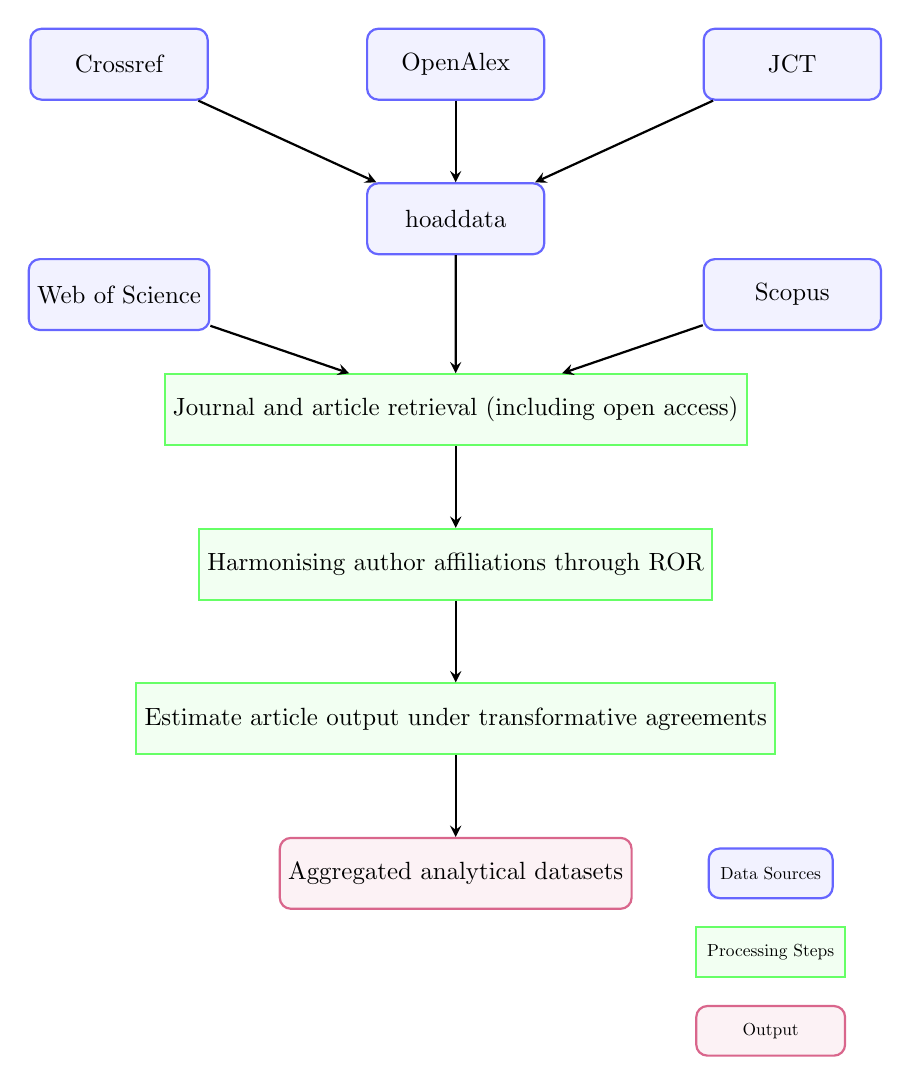
\begin{tikzpicture}[node distance=2cm, thick,scale=1, every node/.style={scale=0.9}]    
% Data Sources
    \node (crossref) [datasource] {Crossref};
    \node (openAlex) [datasource, right=of crossref] {OpenAlex};
    \node (jct) [datasource, right=of openAlex] {JCT};
    \node (wos) [datasource, below=of crossref] {Web of Science};
    \node (scopus) [datasource, below=of jct] {Scopus};
    
    % Processing Steps
    \node (hoaddata) [datasource, below=1.5cm of $(crossref)!1!(openAlex)$] {hoaddata};
    \node (kb) [process, below=1cm of $(wos)!0.5!(scopus)$] {Journal and article retrieval (including open access)};
    
 % Matching Process - Fixed line break syntax
    \node (matching) [process, below=1.5cm of $(hoaddata)!1!(kb)$] {Harmonising author affiliations through ROR};

 % Aggregation
    \node (transmatch) [process, below=1.5cm of $(matching)!1!(matching)$] {Estimate article output under transformative agreements};
        
    % Output
    \node (analysis) [output, below=1.5cm of $(transmatch)!1!(transmatch)$] {Aggregated analytical datasets};
    
    % Arrows
    \draw [arrow] (crossref) -- (hoaddata);
    \draw [arrow] (openAlex) -- (hoaddata);
    \draw [arrow] (jct) -- (hoaddata);
    \draw [arrow] (hoaddata) -- (kb);
    \draw [arrow] (wos) -- (kb);
    \draw [arrow] (scopus) -- (kb);
    \draw [arrow] (kb) -- (matching);
    \draw [arrow] (matching) -- (transmatch);
    \draw [arrow] (transmatch) -- (analysis);

    
    % Legend
    \node [datasource, scale=0.7] at ($(analysis)+(4,0)$) {Data Sources};
    \node [process, scale=0.7] at ($(analysis)+(4,-1)$) {Processing Steps};
    \node [output, scale=0.7] at ($(analysis)+(4,-2)$) {Output};
\end{tikzpicture}
\caption{Data processing workflow for comparing hybrid open access uptake across bibliometric data sources. The workflow shows how data from different sources (hoaddata, derived from Crossref, OpenAlex, Transformative Agreement Data dump used by the cOAlition S Journal Checker Tool (JCT), the Web of Science, and Scopus) were processed to enable comparative analysis.}
\label{fig:workflow}
\end{figure}

\subsection{Data sources}\label{data-sources}

\subsubsection{hoaddata}\label{hoaddata}

hoaddata, developed and maintained by the author to support open access
monitoring and research (e.g. Jahn (2025)), is an R data package that
regularly collects information on hybrid open access uptake from
multiple openly available data sources (Jahn, 2024). It combines
article-level metadata from Crossref (Hendricks et al., 2020) and
affilation metadata from OpenAlex (Priem et al., 2022) with
transformative agreement information from the Transformative Agreement
Data dump used by the cOAlition S Journal Checker Tool (JCT)\footnote{\url{https://journalcheckertool.org/transformative-agreements/}},
which links journal and institutional data about participating research
organisations to agreements in the ESAC registry.

hoaddata follows good practices for computational reproducibility using
R (Marwick et al., 2018). The package, which includes data, code, a test
suite and documentation, is openly available on GitHub. To ensure
computational reproducibility while aggregating the data, a GitHub
Actions continuous integration and delivery (CI/CD) workflow handles
data retrieval from the SUB Göttingen's open scholarly data warehouse
based on Google BigQuery, which provides high-performant programmatic
access to monthly snapshots of Crossref and OpenAlex.\footnote{\url{https://subugoe.github.io/scholcomm_analytics/data.html}}
The workflow has run regularly to fetch updates from these data sources
since 2022. The package version used in this study is 0.3, containing
data from the Crossref 2024-08 dump provided to Crossref Metadata Plus
subscribers and the OpenAlex 2024-08-29 monthly dump. It covers
agreements collected between July 2021 to July 2024 from the JCT. This
version including the computation log is available on GitHub
(https://github.com/subugoe/hoaddata/releases/tag/v.0.3).

\subsubsection{Web of Science}\label{web-of-science}

Clarivate Analytics' Web of Science (WoS) is a well-established
proprietary bibliometric database consisting of several collections
(Birkle et al., 2020). Web of Science is a selective, base
research-focused database (Stahlschmidt \& Stephen, 2022; Visser et al.,
2021). The collections considered in this study were the Science
Citation Index Expanded (SCIE), the Social Sciences Citation Index
(SSCI) and the Arts \& Humanities Citation Index (AHCI).

These collections provides important data points for analysing open
access: author affiliations and roles, differentiation of journal
articles into document types representing different types of journal
contributions, such as original articles or reviews, and open access
status information derived from OurResearch's Unpaywall (Piwowar et al.,
2018), the same provider as OpenAlex. However, the Web of Science lacks
information about journals and articles under transformative agreements.

For programmatic access to article-level data, this study used the
database of the Kompetenznetzwerk Bibliometrie (KB) in Germany. The KB
processes raw XML data provided by Clarivate Analytics, which is
ingested into an in-house PostgreSQL database under a uniform schema. To
support reproducibility, KB maintains annual snapshots of the database.
Accordingly, this study used the annual snapshot from April 2024
(wos\_b\_202404), which is considered to cover almost the entire
previous publication year (Schmidt et al., 2024).

\subsubsection{Scopus}\label{scopus}

Elsevier's Scopus, launched in 2004, is another widely used proprietary
bibliometric database for measuring research (Baas et al., 2020).
Similar to the Web of Science, Scopus is selective with regard to the
journals it indexes. However, its journal coverage is much broader than
that of the Web of Science collections considered in this study, as it
also indexes a wider range of applied research journals (Singh et al.,
2021; Stahlschmidt \& Stephen, 2022; Visser et al., 2021). With detailed
metadata about article types, open access status information derived
from Unpaywall, author roles, and disambiguated affiliations, Scopus
also contains important data to assess open access uptake, although no
direct information regarding transformative agreements was available at
the time of the study.

This study used the Scopus annual snapshot of April 2024 as provided by
the KB (scp\_b\_202404). The same KB curation effort was applied to the
Scopus raw data as for the Web of Science (Schmidt et al., 2024).

\subsection{Data processing steps}\label{data-processing-steps}

\subsubsection{Determining hybrid journal publication
volume}\label{determining-hybrid-journal-publication-volume}

Following Jahn (2025), the starting point was a unified dataset of
several safeguarded JCT snapshots\footnote{\url{https://github.com/njahn82/jct_data}}.
The JCT journal data were enriched with ISSN variants linked to an
ISSN-L. To identify hybrid journals, a comprehensive exclusion of fully
open access journals was performed using multiple journal lists (DOAJ,
OpenAlex, Bielefeld). These data were made available via hoaddata and
used to determine the publication volume of hybrid journals for each
database independently.

hoaddata relies on Crossref for obtaining journal publication volume and
open access status through Creative Commons (CC) licence information
relative to the published version (``version of record''). The article
metadata included DOIs, publication dates, open access information as
well as author roles and affiliations. Publication years were determined
using the earliest known date of publication in a journal. In hoaddata,
this corresponded to Crossref's issued date. For Web of Science and
Scopus, the earliest publication date was used where available, with
Scopus dates specifically determined by the KB through version tracking
of the raw data.

Many transformative agreements typically cover only certain types of
journal articles, in particular original research articles including
reviews (Borrego et al., 2021). Because of limited information on these
document types in open scholarly data (Haupka et al., 2024), hoaddata
used an extended version of Unpaywall's paratext recognition approach to
exclude non-scholarly content (Piwowar et al., 2018). To exclude
conference supplements, which are also often not covered by
transformative agreements, only articles published in regular issues,
indicated by numerical pagination, were considered. For Web of Science
and Scopus, their established, mainly accurate document type
classifications (Donner, 2017; Maisano et al., 2025) were used to
identify original research articles and reviews, referred to as original
articles throughout this study.

\subsubsection{Identifying open access articles in hybrid
journals}\label{identifying-open-access-articles-in-hybrid-journals}

Articles in hybrid journals were considered open access when they were
made freely available under a CC license on publisher platforms. While
hoaddata obtained this information from Crossref license metadata, Web
of Science and Scopus relied on Unpaywall as evidence source. Unpaywall
also uses Crossref license metadata, but supplements them by parsing
publisher websites directly, addressing cases where publishers do not
provide machine-readable CC license information (Piwowar et al., 2018).
This additional parsing remains necessary despite transformative
agreement workflows recommend to deposit CC licenses during DOI
registration (Geschuhn \& Stone, 2017). Both Web of Science and Scopus
defined hybrid open access consistently as content available under CC
licenses on publisher platforms according to their
documentations\footnote{\url{https://webofscience.help.clarivate.com/en-us/Content/open-access.html}}\footnote{\url{https://blog.scopus.com/posts/scopus-filters-for-open-access-type-and-green-oa-full-text-access-option}},
distinguishing it from bronze open access that lack such explicit
license information, or use publisher-specific licenses (Piwowar et al.,
2018).

\subsubsection{Harmonising author affiliations across
databases}\label{harmonising-author-affiliations-across-databases}

Author affiliations were retrieved for both first and, if available,
corresponding authors to prepare the linking between articles and
institutions covered by transformative agreements. To improve the data
retrieval, JCT institution data was enriched with ROR-IDs from
associated institutions, such as university hospitals or institutes of
large research organisations such as the Max Planck Society, according
to OpenAlex' institution entity. To handle different address variants,
database-specific affiliation identifiers were used: ROR-IDs from
OpenAlex for hoaddata, affiliation enhanced names for Web of Science,
and Scopus Affiliation Identifier. Additionally, ISO country codes were
retrieved for each author's address to compile country-level statistics.
These country codes for Web of Science and Scopus were provided by the
KB.

Because neither Web of Science nor Scopus support ROR at the time of the
data retrieval, the institution identifier used by the JCT, a two-step
matching process was implemented to harmonise affiliation data. First,
2,782,540 articles from 6,457 institutions with ROR-IDs in the JCT data
since 2017 (according to hoaddata) were processed to map first authors'
ROR-IDs to corresponding proprietary affiliation identifier in Web of
Science and Scopus using DOI matching. Then, an algorithm selected the
most frequent ROR ID and proprietary identifier pairs to handle multiple
affiliations and organisational hierarchy differences.

This process linked 6,375 ROR IDs to 4,894 Scopus Affiliation IDs, and
6,034 ROR IDs to 2,422 enhanced affiliation strings in the Web of
Science. Quality evaluation through random sampling of 50 pairs revealed
an error rate of 22\% for Web of Science (11 mismatches) and 6\% for
Scopus (3 mismatches). Upon inspection, these mismatches primarily
occurred with less-represented institutions having only a few
publications, introduced through multiple affiliations of single
authors. The difference between databases suggests that Scopus'
affiliation control aligns more closely with ROR than that of the Web of
Science.

\subsubsection{Estimating open access in hybrid journals covered by
transformative
agreements}\label{estimating-open-access-in-hybrid-journals-covered-by-transformative-agreements}

Based on these so-compiled matching tables, articles eligible under
transformative agreements could also be obtained from Web of Science and
Scopus, although they did not contain the ROR IDs used by the JCT. The
estimation of eligible articles followed Jahn (2025) and included a
matching of both journals and participating institutions according to
the JCT. The matching also took into account the duration of agreements
according to the ESAC registry, with only those matches where an
agreement was actually in place being considered for subsequent
analysis. A related study (Jonge et al., 2025), applied to publications
funded by the Dutch Research Council (NWO) and validated against
internal invoicing data, confirmed that such matching can accurately
identify most articles under transformative agreements.

\subsection{Data records}\label{data-records}

As a result of the comprehensive data processing described above,
datasets on open access in hybrid journals included in transformative
agreements were aggregated for each database at country and journal
level by year. Table~\ref{tbl-methods_overview_tab} provides a general
overview of the coverage between 2019 and 2023. It shows that the
majority of hybrid journals published at least one original research
article or review marked as original during the five-year period. These
journals formed the basis for the subsequent calculation of
article-level indicators.

\begin{table}

\caption{\label{tbl-methods_overview_tab}Coverage of hybrid journals in
transformative agreements 2019-23.}

\centering{

\centering
\begin{tabular}[t]{lrrr}
\toprule
\textbf{} & \textbf{hoaddata*} & \textbf{Web of Science} & \textbf{Scopus}\\
\midrule
\addlinespace[0.3em]
\multicolumn{4}{l}{\textbf{Hybrid journal coverage}}\\
\hspace{1em}Active journals & 12,890 & 8,655 & 11,888\\
\hspace{1em}Active journals (core) & 12,888 & 8,655 & 11,878\\
\hspace{1em}Active journals (core) with OA & 11,348 & 8,392 & 11,313\\
\addlinespace[0.3em]
\multicolumn{4}{l}{\textbf{Publication volume}}\\
\hspace{1em}Total published articles & 9,740,015 & 8,616,053 & 8,117,644\\
\hspace{1em}Original articles & 8,158,425 & 6,708,083 & 7,317,703\\
\addlinespace[0.3em]
\multicolumn{4}{l}{\textbf{Digital Object Identifier (DOI) coverage}}\\
\hspace{1em}Articles with DOI & 9,740,015 & 7,713,796 & 8,105,112\\
\hspace{1em}Original articles with DOI & 8,158,425 & 6,695,661 & 7,314,327\\
\addlinespace[0.3em]
\multicolumn{4}{l}{\textbf{Open Access (OA) metrics}}\\
\hspace{1em}OA articles & 998,699 & 1,112,758 & 974,099\\
\hspace{1em}Original OA articles & 969,817 & 1,019,784 & 922,578\\
\addlinespace[0.3em]
\multicolumn{4}{l}{\textbf{Original articles with affiliation data}}\\
\hspace{1em}First author articles & 7,242,542 & 6,294,855 & 7,232,017\\
\hspace{1em}Corresponding author articles & 5,534,207 & 6,291,441 & 6,898,487\\
\bottomrule
\multicolumn{4}{l}{\rule{0pt}{1em}\textsuperscript{*} Journal article metadata from Crossref, except affiliations from OpenAlex}\\
\end{tabular}

}

\end{table}%

While hoaddata only covers articles with a DOI, Scopus and Web of
Science publication indicators were calculated using their database
identifier. A subsequent comparison of DOI coverage shows that
non-original articles in Web of Science often lacked a DOI. This was
particularly the case for meeting abstracts, which are notably prevalent
in Health Sciences journals (Melero-Fuentes et al., 2025) and are not
indexed by Scopus (Donner, 2017). Open access indicators were aggregated
by DOI, as Unpaywall only collects information on open access status for
articles with a DOI. A closer look at original articles with affiliation
data, and in line with related research (Zhang et al., 2024), reveals a
lack of affiliation data in the case of OpenAlex, the affiliation data
source used by hoaddata, compared to Web of Science and Scopus. In
particular, only about two-thirds of the articles examined provided
corresponding author affiliations. For first authors, the proportion was
89\%. At the time of writing, OpenAlex disclosed limited coverage of
corresponding authorhip data \footnote{\url{https://docs.openalex.org/api-entities/works/work-object/authorship-object\#is_corresponding}}.
Therefore, only first author data for hoaddata were considered in the
following analysis.

\subsection{Data analysis}\label{data-analysis}

Throughout this largely automated data collection and analysis process,
Tidyverse tools (Wickham et al., 2019) for the R programming language (R
Core Team, 2024) were used. Rank correlations were calculated using the
Hmisc package (Harrell Jr, 2003). The source code analysis, including
all queries used to obtain the data, is available on GitHub (add link).
An interactive supplement exploring correlations between the data
sources examined by country and publisher is available on HuggingFace
Spaces: https://huggingface.co/spaces/najkoja/hoa\_replication.

\section{Results}\label{results}

This section first presents the indexing coverage of hybrid open access
by comparing open data sources with the proprietary bibliometric
databases Scopus and Web of Science. Then, using the same methods,
indicators at the publisher and country level are calculated
independently for each database and compared with each other to assess
the suitability of the bibliometric databases for investigating
transformative agreements.

\subsection{Coverage comparision}\label{coverage-comparision}

\subsubsection{Overview}\label{overview}

Figure \ref{fig-upset_coverage_results} presents the coverage of hybrid
journals included in transformative agreements, visualising the
intersections of journals and articles across the examined databases as
an UpSet graph (Krassowski, 2020; Lex et al., 2014). The analysis
included hybrid journals that published at least one open access article
between 2019 and 2023, based on open access status information from each
database. Only original research articles and reviews were considered in
the analysis.

\begin{figure}[ht!]

\centering{

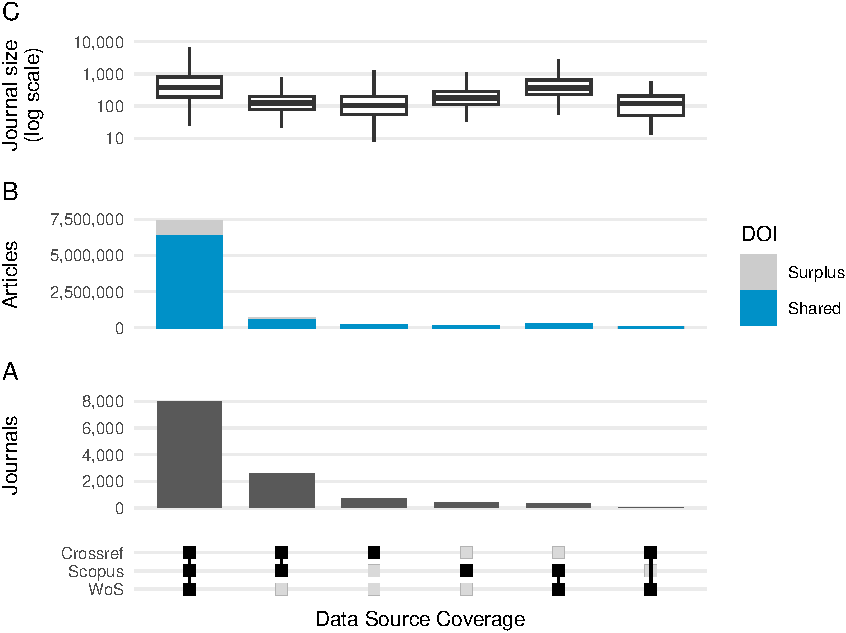
\includegraphics[width=0.99\linewidth,height=\textheight,keepaspectratio]{fig/fig-upset_coverage_results-1.pdf}

}

\caption{\label{fig-upset_coverage_results}Comparison of the hybrid open
access indexing coverage of hoaddata (based on Crossref), Scopus and Web
of Science, 2019-2023. Only hybrid journals present in the cOAlition S
Transformative Agreement Data dump with at least one open access article
are considered. A) presents the number of journals, B) the number of
articles (DOI), distinguishing between shared DOI corpus and surplus in
hoaddata. Box plots (C) shows the five-years journal article volume
(log-scale).}

\end{figure}%

Journal coverage analysis revealed that 66\% (n = 7,970) of hybrid
journals included in transformative agreements were indexed in all three
databases (Figure \ref{fig-upset_coverage_results}A). The second-largest
set consisted of journals indexed in both hoaddata and Scopus,
comprising 21\% (n = 2,595) of hybrid journals. Notably, 6\% (n = 739)
of journals were exclusively contained in hoaddata, while another 6\% (n
= 748) were only found in the proprietory database Scopus. Of these, 354
were also available in the Web of Science. Upon inspection, this group
of hybrid journals exclusively covered in the proprietary data sources
mainly represented hybrid journals for which no open access evidence
could be retrieved from Crossref, the open access evidence source for
hoaddata.

In terms of article coverage, Figure \ref{fig-upset_coverage_results}B
shows the total publication volume per combination in terms of DOI
availability. The largest set of hybrid journals, which includes all
three data sources, also contains the largest number of articles. In
total, these journals recorded 6,289,687 overlapping articles,
represented by the blue bar. They represented 94\% of original articles
with DOI indexed in the Web of Science sample, and 86\% in Scopus.
Another 657,697 articles were exclusive to both Scopus and hoaddata.
Exclusively in hoaddata were 177,110 articles, and exclusively in the
proprietary databases were 325,194 articles.

Figure \ref{fig-upset_coverage_results}B also shows the surplus of
articles with DOI that were only available via hoaddata (grey area). In
case of hybrid journals covered by all three data sources, 1,023,882
DOIs were only present in hoaddata. After validation at the DOI level
using the KB databases and manual inspection, the main reasons for
missing DOI coverage in the proprietary database were insufficient
classification of journal content as original research articles and
reviews during the compilation of hoaddata. Particularly, letters and
editorials could not be fully detected. Paratext recognition failed in
37\% of DOIs to identify non-scholarly content such as front matters or
reviewer lists, which are generally not indexed by Scopus and Web of
Science. To a lesser extent, differences in publication and indexing
dates were a reason for non-overlapping DOIs.

Using overlapping DOIs, the publication volume between 2019 and 2023 was
also calculated for each journal. Figure
\ref{fig-upset_coverage_results}C illustrates the distribution for each
combination. It shows a large spread across the journals jointly covered
by all three data sources. These journals published more on average than
journals covered by only one or two data sources. In particular, the
journals covered exclusively by hoaddata were substantially smaller.
Upon inspection, these were often newly launched hybrid journals, which
explains the relatively low five-year publication volume. An example is
\emph{Digital society} that published 86 articles. This hybrid journal
was launched in 2022, being covered by various Springer Nature
transformative agreements since then.

\subsubsection{Coverage by publisher
portfolio}\label{coverage-by-publisher-portfolio}

Figure \ref{fig-upset_coverage_results_publisher} presents the coverage
of hybrid journals in transformative agreements across data sources from
2019 to 2023 with a focus on publisher portfolios. The analysis
highlights the dominance of the three largest publishers, Elsevier,
Springer Nature, and Wiley, which collectively accounted for 47\% of
hybrid journals and 62\% of articles published during this five-year
period. In terms of article volume, Elsevier led with 2,441,358 articles
(33\% of the total) published across 1,951 hybrid journals (16\% of the
total). Springer Nature followed with 1,247,578 articles (17\%) in
2,311, although recording the largest number of hybrid journals (19\%).
Wiley accounted for 858,939 articles (12\%) in 1,382 hybrid journals
(11\%). The remaining 54 publishers collectively accounted for 2,749,847
articles (38\%) in 6,476 hybrid journals (53\%).

\begin{figure}[ht!]

\centering{

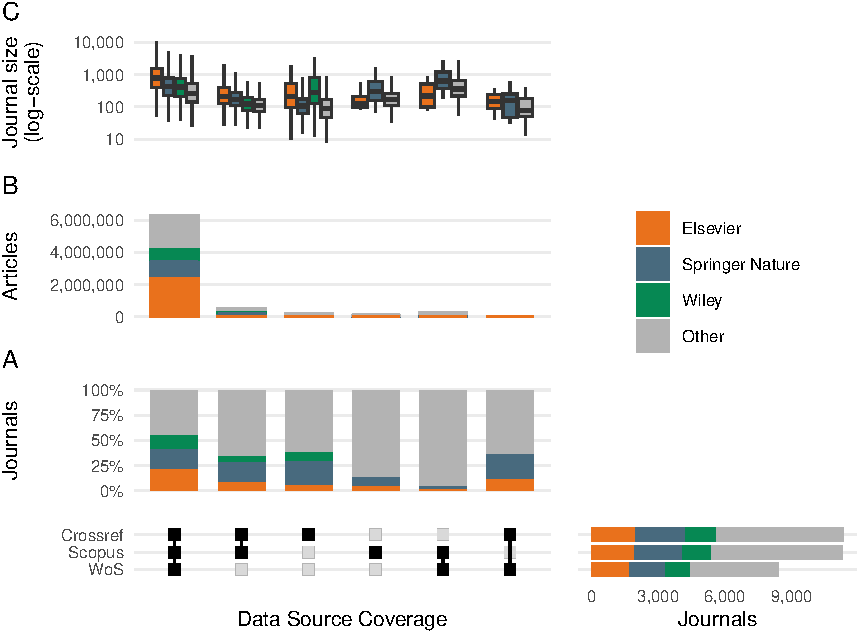
\includegraphics[width=0.99\linewidth,height=\textheight,keepaspectratio]{fig/fig-upset_coverage_results_publisher-1.pdf}

}

\caption{\label{fig-upset_coverage_results_publisher}Comparison of the
hybrid open access indexing coverage of hoaddata (based on Crossref),
Scopus and Web of Science, 2019-2023 by publisher. Only hybrid journals
present in the cOAlition S Transformative Agreement Data dump with at
least one open access article are considered. A) presents the percentage
of journals by publisher, B) the number of articles by publisher (shared
DOI). Box plots (C) shows the five-years journal article volume
(log-scale) by publisher.}

\end{figure}%

The three largest publishers, Elsevier, Springer Nature, and Wiley, were
best represented in the exclusive intersection of all three data sources
(hoaddata, Scopus, and Web of Science). Together, they comprised 4,384
hybrid journals (55\% of the intersectional set) and dominated article
coverage (n = 4,174,315; 66\%), as determined through shared DOIs. When
examining publication volume per journal, (Figure
\ref{fig-upset_coverage_results_publisher}C), Elsevier published, on
average, the largest journals, followed by Springer Nature and Wiley.

Comparing publisher portfolios across different indexing sets
demonstrates that publisher were not represented uniformly. Notably,
Springer Nature exhibited 519 hybrid journals exclusively indexed in
both hoaddata and Scopus. This set included journals from the Chinese
Academy of Science, German-language medical journals, and Eastern
European publications including the \emph{Journal of Mathematical
Sciences}, which also publishes English-language translations of
Russian-language works. Additionally, this subset included titles with a
more broader disciplinary focus such as \emph{SN Computer Science} and
newly launched hybrid journals like \emph{Nature Computational Science},
which started in 2021 and was indexed in Scopus but not yet in Web of
Science. The set also captured ceased journals, providing further
insights into the dynamics of journal publishing.

Examining publisher portfolios not covered by hoaddata but present in
Scopus or Web of Science identified several publishers with missing CC
license information in Crossref. In particular, Emerald represented 322
journals with 86,409 articles, AIP Publishing accounted for 24 journals
with 64,898 articles, and World Scientific recorded 87 journals and
42,531 articles. In total, 9 publishers did not share CC licenses with
Crossref and were therefore not represented in hoaddata.

An inspection of individual journals also uncovered discrepancies in
Unpaywall's open access identification for certain publishers that
typically deposit CC licenses with Crossref. Notably, some
subscription-only journals contained one or two articles erroneously
tagged as hybrid open access by Unpaywall, which were subsequently
reflected in Scopus and Web of Science. Examples of such
misclassifications include Elsevier's \emph{Journal of Bioscience and
Bioengineering} and Springer Nature's \emph{Journal of Mechanical
Science and Technology}.

\subsection{Open Access Indicator
Comparision}\label{open-access-indicator-comparision}

This section examines the uptake of open access in hybrid journals,
focusing on the influence of transformative agreements across hoaddata,
Scopus, and Web of Science. The aim was to assess whether consistent
results can be derived from these data sources despite differences in
coverage and methodologies. Following Jahn (2025), indicators were
calculated for each data source and comprise the number and proportion
of open access articles, including those enabled by transformative
agreements, from 2019 to 2023. For Web of Science and Scopus, the impact
of transformative agreements was estimated using both first and
corresponding authorships, while hoaddata indicator calculation was
limited to first author affiliations.

\begin{figure}[ht!]

\centering{

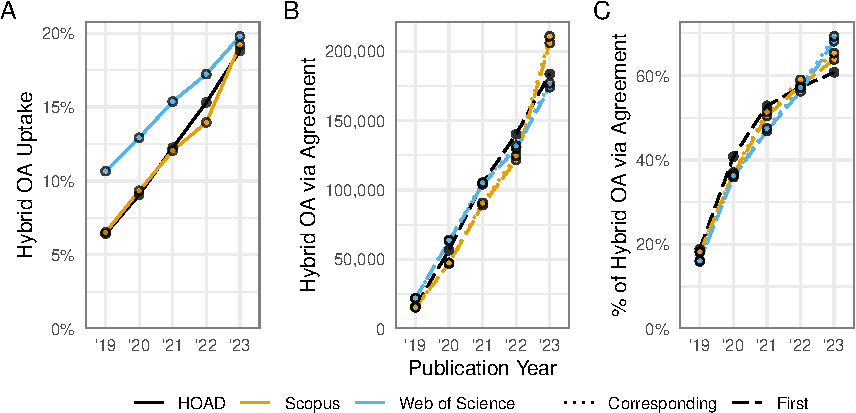
\includegraphics[width=0.99\linewidth,height=\textheight,keepaspectratio]{fig/fig-uptake_overview-1.pdf}

}

\caption{\label{fig-uptake_overview}Development of open access in hybrid
journals included in transformative agreements, 2019 and 2023 by data
source and author role. Figure shows the open access percentage (A), the
number (B) and percentage (C) of open access articles enabled
transformative agreements.}

\end{figure}%

\subsubsection{Overview}\label{overview-1}

Figure \ref{fig-uptake_overview}A shows a moderate growth of open access
in hybrid journals, which is consistent across hoaddata (black line),
Scopus (yellow line), and Web of Science (blue line). According to
hoaddata, hybrid open access uptake increased from 6.4\% (n = 85,071) in
2019 to 19\% (n = 302,358) in 2023. Similarly, Scopus recorded an growth
from 6.5\% (n = 84,648) in 2019 to 19\% (n = 322,850) in 2023. However,
Web of Science recorded higher open access uptake in early years, before
converging in 2023, from 11\% (n = 137,202) in 2019 to 20\% (n =
255,481) in 2023, suggesting an different approach towards labeling
hybrid open access by the Web of Science.

Similarly, hybrid open access by transformative agreements increased
between 2019 and 2023 (Figures \ref{fig-uptake_overview}B and C). Trends
were consistent when measuring first (dashed line) and corresponding
author (dotted line) affiliations. According to Scopus, 479,297 open
access articles could be attributed to transformative agreements based
on first author metadata (increasing from 15,341 to 206,084) and 489,262
using corresponding author metadata (from 15,444 to 210,816). Web of
Science recorded 493,028 open access articles via transformative
agreements using first author metadata (increasing from 21,871 to
174,126) and 500,076 using corresponding author metadata (from 22,092 to
177,030). hoaddata, lacking corresponding author data, linked 0 articles
to transformative agreements but showed slower growth than Scopus and
Web of Science, from 0 in 2019 to 0 in 2023.

From 2021 (hoadata, Scopus) resp. 2022 (Web of Science), transformative
agreements enabled the majority of hybrid open access. For first
authors, the share ranged between 61\% (hoaddata), 64\% (Scopus), and 68
\% (Web of Science) in 2023. For corresponding authors, the shares were
slightly larger, with Scopus recording 65\% and Web of Science 69\% in
2023. However, substantial hybrid open access was still facilitated
outside transformative agreements, likely through APCs paid from
discretionary research funds (Jahn et al., 2022; Suber, 2012).

\subsubsection{Open access by
publishers}\label{open-access-by-publishers}

\begin{figure}[ht!]

\centering{

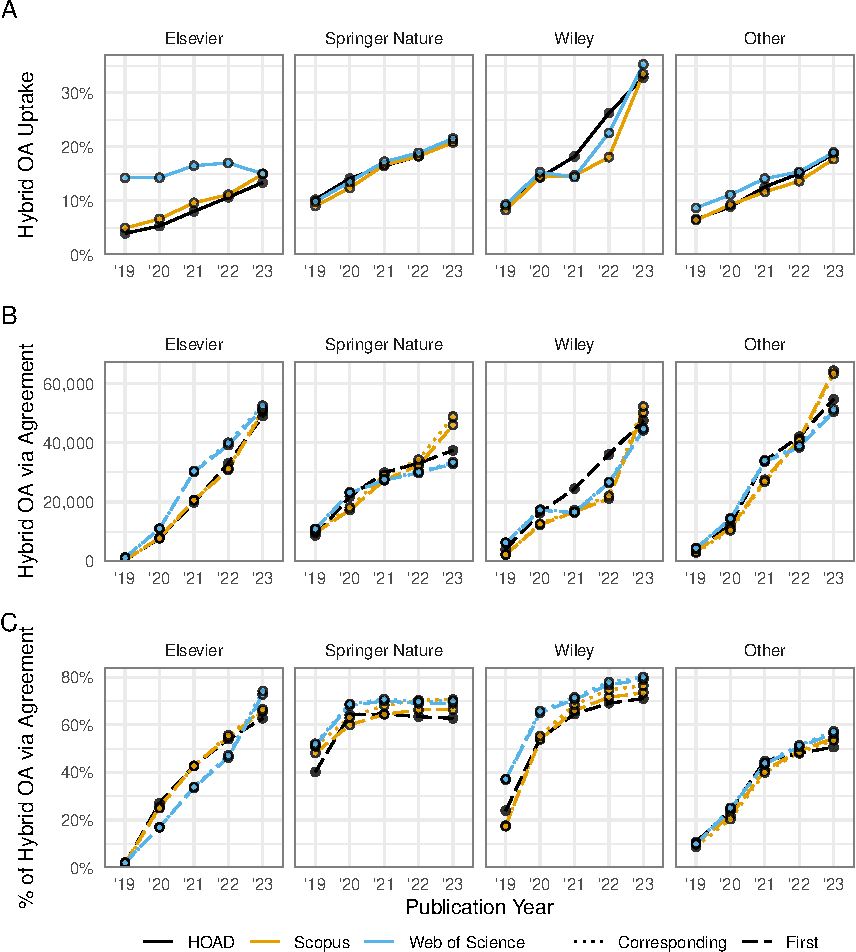
\includegraphics[width=0.99\linewidth,height=\textheight,keepaspectratio]{fig/fig-uptake_publisher-1.pdf}

}

\caption{\label{fig-uptake_publisher}Development of open access in
hybrid journals included in transformative agreements, 2019 and 2023, by
data source, author role and publisher. Figure shows the open access
percentage (A), the number (B) and percentage (C) of open access
articles enabled transformative agreements.}

\end{figure}%

When considering open access trends by publisher (see Figure
\ref{fig-uptake_publisher}), the observed differences in early uptake
rates between hoaddata and Scopus compared to Web of Science can be
largely attributed to articles published in Elsevier hybrid journals,
the largest publisher in our sample. Both hoadata and Scopus reported an
steady increase in open access uptake between 2019 and 2023 (hoaddata
from 4\% to 13\%; Scopus from 5\% to 15\%). In contrast, Elsevier's
share remained relatively constant, increasing only slightly from 14\%
to 15\% according to the Web of Science. Upon inspection, this
discrepancy primarily stemmed from articles in the publisher's open
archive. These articles, made freely available after an embargo period
under Elsevier's user license, were tagged as hybrid open access in Web
of Science, even though its documentation\footnote{\url{https://webofscience.help.clarivate.com/en-us/Content/open-access.html}}
specified that only articles under a CC license variant were considered.
Previous research (Haustein et al., 2024; Jahn et al., 2022) has shown
that Elsevier provided a substantial portion of its articles under this
license, explaining the relatively large and stable share of open access
over the years.

Differences in open access evidence are also evident for Wiley.
Specifically, Web of Science and Scopus recorded a drop in 2021 and 2022
compared to hoaddata. For these two years, hoaddata reported 35,308 more
open access articles than Scopus and 32,491 more than Web of Science.
This discrepancy is presumably because of challenges in fetching
full-texts by Unpaywall, the open access evidence source for Scopus and
Web of Science. According to Unpaywall's software version history,
Wiley's publisher platform redirects prevented Unpaywall from parsing
license information from full-texts.\footnote{See Unpaywall version
  history related to Wiley fixes:
  \url{https://github.com/search?q=repo\%3Aourresearch\%2Foadoi+wiley&type=commits}}
hoaddata, which relies solely on Crossref metadata for open access
identification, was unaffected by these issues.

Despite these differences in open access evidence, the three data
sources show consistent temporal trends in hybrid open access enabled by
transformative agreements (see Figure \ref{fig-uptake_publisher}B and
C). Wiley emerged as the fastest-growing publisher in terms of open
access uptake, with more than 30\% of articles in hybrid journals
reported as open access in 2023 across the examined data sources,
followed by Springer Nature and Elsevier, recording a comparable late
uptake, which is consistent with the publisher's historical reluctance
to engage in negotations with library consortia. However, by 2023, the
share of open access enabled by transformative agreements appeared to
stabilise for all three publishers (see Figure
\ref{fig-uptake_publisher}C). Interestingly, the differences between
first and corresponding author affiliations were more pronounced at the
publisher level. In Scopus, for example, the share of open access via
transformative agreements measured by corresponding authorship was
greater for Springer Nature in 2023 than when using first authorship.

\subsubsection{Open access by country}\label{open-access-by-country}

When comparing countries, consistent patterns were observed across data
sources for the five-year period 2019 to 2023. Figure
\ref{fig-uptake_country} presents hybrid open access indicators by
country, comparing hoaddata (x-axis) with Web of Science and Scopus
(y-axis). Indicators calculated from these proprietary databases are
shown for both first and corresponding authors, with full counting used
to account for multiple country affiliations (Hottenrott et al., 2021).

\begin{figure}[ht!]

\centering{

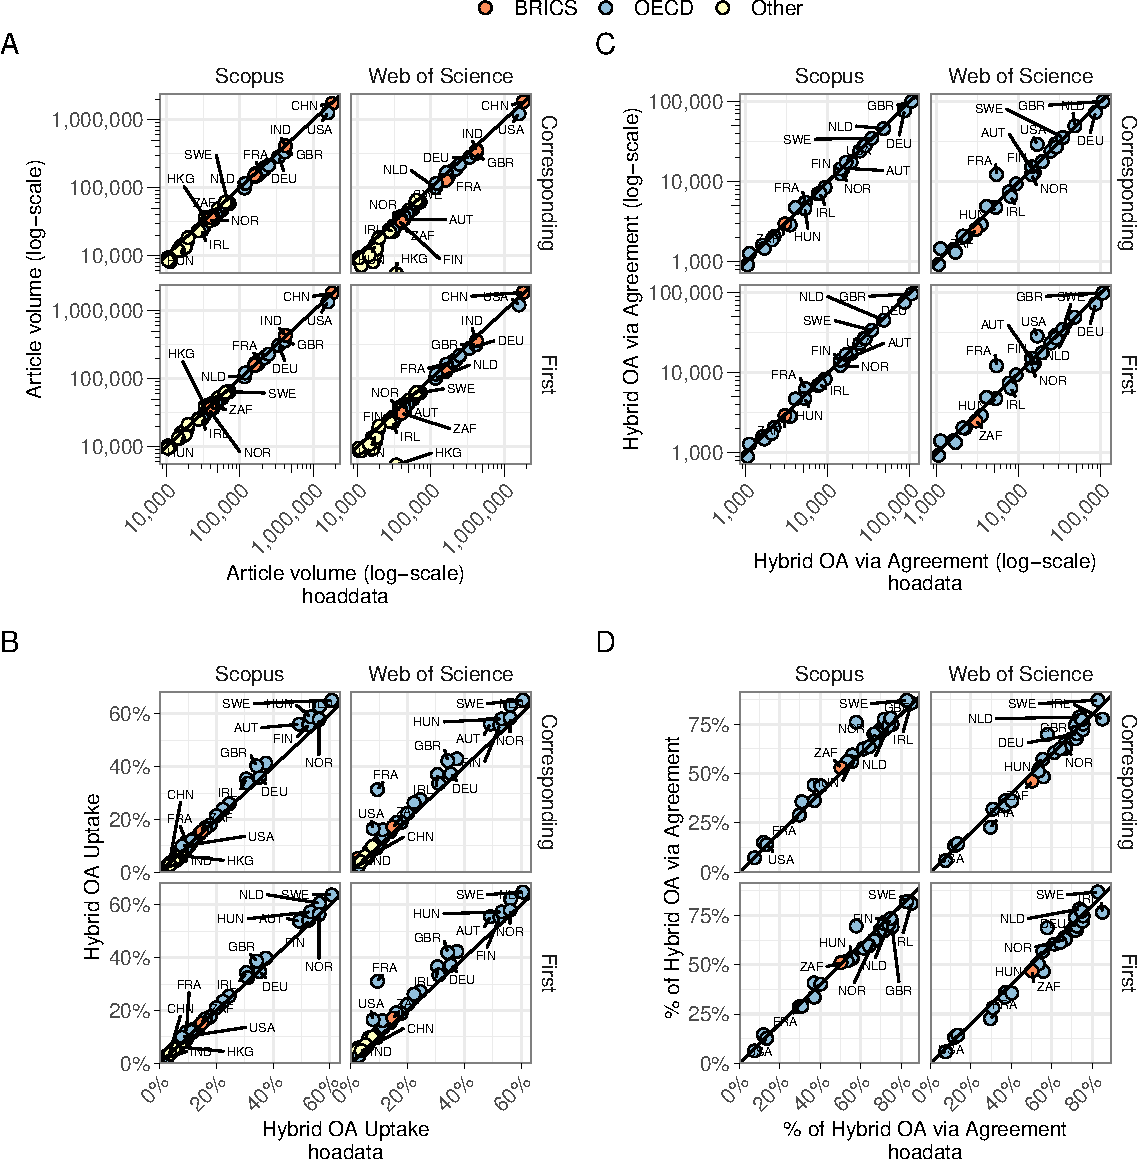
\includegraphics[width=0.99\linewidth,height=\textheight,keepaspectratio]{fig/fig-uptake_country-1.pdf}

}

\caption{\label{fig-uptake_country}Comparison of hybrid open access by
country, 2019-2023. Scatterplots distinguish between proprietary
database Scopus and Web of Science, and author role. x axis shows
hoaddata indicators. A) Five-years article volume, B) open access
percentage in hybrid journals, (A and B limited to countries with
\textgreater{} 10.000 articles published), C) number and D) percentage
of open access articles enabled by transformative agreements (limited to
countries with \textgreater{} 1.000 open access articles enabled by
transformative agreements). Line represents line of equality. An
interactive version is accessible here:
\url{https://najkoja-hoa-replication.hf.space/}}

\end{figure}%

In terms of article output by country (see Figure
\ref{fig-uptake_country}A), strong positive correlation was observed
across the data sources and author roles (Spearman rank correlation
\(\rho > .9\), \(p < 0.001\)). Between 2019 and 2023, China was the most
productive country, followed by the United States and, by a certain
margin, India, the United Kingdom, and Germany. Analysis of authorship
roles revealed minimal variation, indicating that first and
corresponding authors were typically from the same country.

When examining the percentage of open access articles in hybrid journals
(see Figure \ref{fig-uptake_country}B), a different pattern emerged.
Authors affiliated with institutions from medium-sized European
countries, such as Sweden, the Netherlands, Finland, and Hungary,
provided a large proportion of their articles in open access. Germany
and the United Kingdom also had approximately 40\% of their output
available as open access. In contrast, non-OECD countries showed notably
lower adoption of hybrid open access, with South Africa being the only
BRICS member well-represented in the data. The United States also
demonstrated a relatively low proportion of open access articles. These
findings were consistent across all databases. However, France was
better represented in Web of Science, likely due to its agreement with
Elsevier starting in 2019, which allowed delayed open access under the
publisher's user license (Rabesandratana, 2019). This licence was not
classified as hybrid open access in either Scopus or hoaddata. In all
cases, Spearman rank correlations were \(\rho > .9\), \(p < 0.001\),
showing a high level of correlations between the databases and
authorship roles considered.

Transformative agreements appeared to be a key driver of national open
access growth (see Figure \ref{fig-uptake_country}C and D). OECD members
accounted for the majority of open access articles enabled by
transformative agreements. As a notable exception, South Africa also
featured prominently, as the South African National Library and
Information Consortium (SANLiC) successfully negotiated transformative
agreements with major publishers from 2022 onward.\footnote{\url{https://sanlic.ac.za/read-and-publish-agreements/}}
Results were consistent across data sources. However, Wiley's open
access surplus in hoaddata led to better rankings for countries where
Wiley played a substantial role, such as Germany, where the DEAL
consortium negotiated its first transformative agreements with publisher
that started in July 2019.

Medium-sized European countries again showed a high proportion of hybrid
open access through transformative agreements (see Figure
\ref{fig-uptake_country}D), highlighting the impact of this licensing
model across all three data sources. In contrast, the United States had
a low proportion of hybrid open access enabled by agreements, suggesting
that a substantial number of open access articles from US-based authors
were likely financed through other means.

In all cases, strong positive correlations were observed using
Spearman's rank correlation: \(\rho > .9\), \(p < 0.001\) between data
sources and authorship roles, when considering countries with an minimum
of 1,000 open access articles enabled by transformative agreements
between 2019 and 2023. When this limitation was removed, the correlation
remained strong but slightly lower (\(\rho > .85\), \(p < 0.001\)). This
difference may signal countries where only a few institutions had
transformative agreements in place, as opposed to those participating in
national consortia with broader participation.

\section{Discussion}\label{discussion}

This study of over 13,000 hybrid journals shows a rise in open access
due to transformative agreements between 2019 and 2023, although most
articles remained paywalled. While transformative agreements accounted
for the majority of open access, many articles continue to become open
through the payment of individual publication fees. Hybrid open access
and transformative agreements remain concentrated among a small group of
large commercial publishers, with high-income European
countries---alongside South Africa---showing high adoption rates. In
contrast, the three most productive countries, China, the United States,
and India, were substantially ranked lower in transformative agreement
adoption. Open questions remain whether this uneven distribution
reflects temporary implementation gaps, inherent inequities in the
transformative agreement model, or a deliberate avoidance of such
agreements.

The findings were consistent across the investigated open data source
hoaddata, derived from Crossref and OpenAlex, and the established
proprietary bibliometric databases Scopus and Web of Science. Notably,
and aligning with previous studies (Akbaritabar et al., 2024; Alperin et
al., 2024) and rankings (N. J. van Eck et al., 2024), the results show
strong correlations by country affiliation, which supports using open
metadata for large-scale analyses of hybrid open access. However, the
observed differences in journal coverage and metadata availability
warrant discussion, affecting not only open data sources but also
proprietary databases when used in isolation.

The coverage analysis reveals that hybrid journals are well indexed in
all three data sources, particularly in terms of article coverage,
reflecting the dominance of major publishers whose established journal
portfolios are comprehensively indexed in proprietary databases (Bellen
et al., 2024). Differences emerge for journals targeting practitioners
or local non-English language communities, with many such titles indexed
exclusively in Crossref and Scopus. Using Crossref as a bibliometric
database in hoaddata demonstrated particular strength in identifying
newly established hybrid journals, a notable finding given that
transformative agreements primarily target existing subscription-based
journals. The landscape of hybrid journal publishing thus differs
markedly from that of fully open access journals. Comparing the coverage
of OpenAlex, Scopus and Web of Science, Simard et al. (2024) indicate
that only half of the fully open access journals listed in the DOAJ are
also indexed in Scopus and Web of Science. Notably, journals that charge
no publication fees (``diamond journals'') are absent from the selective
Web of Science, which reinforces existing disparities in the indexing of
under-represented research communities and regions in selective
bibliometric databases (Simard et al., 2024)

A frequently reported limitation of studying open access with less
selective databases is the lack of corresponding authorship information
(Fraser et al., 2023; Haucap et al., 2021; Shu \& Larivière, 2023).
However, this analysis demonstrates that indicators based on first
authors, which have often been used as a proxy for determining open
access funding, and corresponding authors show a high level of
correlation, reflecting disciplinary norms in scholarly publishing with
regard to contributorship and author roles and positions (Larivière et
al., 2016). First authors typically conduct the main research underlying
a paper, while the corresponding author often supervises the research
(Fox et al., 2018; Mattsson et al., 2010). Unsurprisingly, measures
based on first or corresponding authorships are strongly correlated,
suggesting that these authors share the same country affiliation.
Moreover, in most cases, the first author is identical to the
corresponding author (Chinchilla-Rodríguez et al., 2024). Despite this
correlation, the study observed a recent slight increase in open access
articles by corresponding authors over first authors across Springer
Nature hybrid journals prompts questions about how institutional open
access sponsorship practices influence author roles and assignments
within co-author teams, especially as funding opportunities vary
(Gumpenberger et al., 2018). Previous research has highlighted how
institutionalized bibliometric practices can affect the valuation of
authorship positions (Helgesson, 2020), suggesting the need to monitor
potential influences of the availability of open access funding on
authorships (Maddi \& Silva, 2024).

Another critical data element in the study is affiliation data, which is
essential for estimating open access enabled by transformative
agreements. Although OpenAlex's affiliation coverage is less
comprehensive, which likely reduced the number of articles confidently
attributed to transformative agreements in this study, it still shows
high correlations with Scopus and Web of Science at the country level.
However, OpenAlex's native ROR ID integration offers a distinct
advantage, enabling more reliable identification of agreement-enabled
articles compared to Scopus and Web of Science, which require
reconciliation with proprietary organization identifiers. Future studies
based on the Web of Science will benefit from the recent integration of
ROR-IDs, announced by the end of 2024.

The database comparison revealed important discrepancies in open access
evidence. Crucially, not all publishers deposit CC licences with
Crossref, a limitation that becomes apparent when contrasting Crossref
with Unpaywall's data in Scopus and Web of Science. While Unpaywall can
detect such gaps by parsing publishers' websites for open access
licences, it nevertheless missed a substantial number of CC-licensed
open access articles from Wiley journals indexed in Crossref, likely due
to parsing errors on the publisher's website. This resulted in fewer
open access articles being recorded in Scopus and Web of Science.
Further inconsistencies emerged between Scopus and Web of Science,
despite both relying on Unpaywall: Web of Science erroneously labels
Elsevier's delayed open access as hybrid, whereas Scopus correctly
categorises it. Notably, Scopus and Crossref showed greater alignment
than observed in a related comparison between Scopus and OpenAlex
(Alperin et al., 2024). This likely reflects the use of a curated list
to identify hybrid open access journals, rather than relying solely on
article-level tags. Given these variations, which may compromise
comparability, research and monitoring exercises should avoid reliance
on a single source. Instead, the selection of open access evidence
should be cross-verified using multiple sources and snapshots that can
be used to track changes in the data over time (Huang et al., 2020).
Incorporating expert-curated journal lists can also help prevent
misclassification based on business models (Visser et al., 2021).

It is important to note that the study's estimates of articles from
institutions involved in transformative agreements are approximations
due to a lack of access to invoice data, which is not usually shared by
library consortia and publishers. Furthermore, the data sources about
transformative agreements including the cOAlition S Journal Checker Tool
and the ESAC registry are a voluntary effort, crowd-sourced from various
consortia. However, recent validation with Dutch research information
demonstrates the reliability of such an open approach for the assessment
of articles under transformative agreements (Jonge et al., 2025). With
enhanced open metadata compliance, attributable to evolving standards
and initiatives to support negotiations with publishers, particularly
through the communities of the ESAC initiative and Barcelona Declaration
supporters, the situation is likely to improve. In conclusion, this
study has shown that open metadata are suitable for analysing the
transition from subscription-based journal publishing to full open
access.

\section{References}\label{references}

\phantomsection\label{refs}
\begin{CSLReferences}{1}{0}
\bibitem[\citeproctext]{ref-Akbaritabar_2024}
Akbaritabar, A., Theile, T., \& Zagheni, E. (2024). Bilateral flows and
rates of international migration of scholars for 210 countries for the
period 1998-2020. \emph{Scientific Data}, \emph{11}(1).
\url{https://doi.org/10.1038/s41597-024-03655-9}

\bibitem[\citeproctext]{ref-alperin2024analysissuitabilityopenalexbibliometric}
Alperin, J. P., Portenoy, J., Demes, K., Larivière, V., \& Haustein, S.
(2024). An analysis of the suitability of OpenAlex for bibliometric
analyses. \emph{arXiv}. \url{https://arxiv.org/abs/2404.17663}

\bibitem[\citeproctext]{ref-Aspesi_2020}
Aspesi, C., \& Brand, A. (2020). In pursuit of open science, open access
is not enough. \emph{Science}, \emph{368}(6491), 574--577.
\url{https://doi.org/10.1126/science.aba3763}

\bibitem[\citeproctext]{ref-Baas_2020}
Baas, J., Schotten, M., Plume, A., Côté, G., \& Karimi, R. (2020).
Scopus as a curated, high-quality bibliometric data source for academic
research in quantitative science studies. \emph{Quantitative Science
Studies}, \emph{1}(1), 377--386.
\url{https://doi.org/10.1162/qss_a_00019}

\bibitem[\citeproctext]{ref-budapest}
Babini, D., Chan, L., Hagemann, M., Joseph, H., Kuchma, I., \& Suber, P.
(2022). \emph{{The Budapest Open Access Initiative-20th. Anniversary
recommendations (BOAI20)}}.
\url{https://www.budapestopenaccessinitiative.org/boai20/}

\bibitem[\citeproctext]{ref-Bakker_2024}
Bakker, C., Langham-Putrow, A., \& Riegelman, A. (2024). Impact of
transformative agreements on publication patterns: An analysis based on
agreements from the ESAC registry. \emph{International Journal of
Librarianship}, \emph{8}(4), 67--96.
\url{https://doi.org/10.23974/ijol.2024.vol8.4.341}

\bibitem[\citeproctext]{ref-vanbellen2024oligopolyacademicpublisherspersists}
Bellen, S. van, Alperin, J. P., \& Larivière, V. (2024). \emph{The
oligopoly of academic publishers persists in exclusive database}.
\url{https://arxiv.org/abs/2406.17893}

\bibitem[\citeproctext]{ref-Birkle_2020}
Birkle, C., Pendlebury, D. A., Schnell, J., \& Adams, J. (2020). {Web of
Science} as a data source for research on scientific and scholarly
activity. \emph{Quantitative Science Studies}, \emph{1}(1), 363--376.
\url{https://doi.org/10.1162/qss_a_00018}

\bibitem[\citeproctext]{ref-Borrego_2020}
Borrego, Á., Anglada, L., \& Abadal, E. (2021). Transformative
agreements: Do they pave the way to open access? \emph{Learned
Publishing}, \emph{34}(2), 216--232.
\url{https://doi.org/10.1002/leap.1347}

\bibitem[\citeproctext]{ref-Jisc_2024}
Brayman, K., Devenney, A., Dobson, H., Marques, M., \& Vernon, A.
(2024). \emph{A review of transitional agreements in the {UK}}. Zenodo.
\url{https://doi.org/10.5281/zenodo.10787392}

\bibitem[\citeproctext]{ref-Butler_2023}
Butler, L.-A., Matthias, L., Simard, M.-A., Mongeon, P., \& Haustein, S.
(2023). The oligopoly's shift to open access: How the big five academic
publishers profit from article processing charges. \emph{Quantitative
Science Studies}, \emph{4}(4), 778--799.
\url{https://doi.org/10.1162/qss_a_00272}

\bibitem[\citeproctext]{ref-ifla}
Campbell, C., Dér, Á., Geschuhn, K., \& Valente, A. (2022). How are
transformative agreements transforming libraries? \emph{87th IFLA World
Library and Information Congress (WLIC) / 2022 in Dublin, Ireland}.
\url{https://repository.ifla.org/handle/123456789/1973}

\bibitem[\citeproctext]{ref-C_spedes_2025}
Céspedes, L., Kozlowski, D., Pradier, C., Sainte‐Marie, M. H., Shokida,
N. S., Benz, P., Poitras, C., Ninkov, A. B., Ebrahimy, S., Ayeni, P.,
Filali, S., Li, B., \& Larivière, V. (2025). Evaluating the linguistic
coverage of {OpenAlex}: An assessment of metadata accuracy and
completeness. \emph{Journal of the Association for Information Science
and Technology}. \url{https://doi.org/10.1002/asi.24979}

\bibitem[\citeproctext]{ref-Chinchilla_Rodr_guez_2024}
Chinchilla-Rodríguez, Z., Costas, R., Robinson-García, N., \& Larivière,
V. (2024). Examining the quality of the corresponding authorship field
in {Web of Science} and {Scopus}. \emph{Quantitative Science Studies},
\emph{5}(1), 76--97. \url{https://doi.org/10.1162/qss_a_00288}

\bibitem[\citeproctext]{ref-culbert2024referencecoverageanalysisopenalex}
Culbert, J., Hobert, A., Jahn, N., Haupka, N., Schmidt, M., Donner, P.,
\& Mayr, P. (2024). \emph{Reference coverage analysis of OpenAlex
compared to web of science and scopus}.
\url{https://arxiv.org/abs/2401.16359}

\bibitem[\citeproctext]{ref-D_r_2025}
Dér, Á. (2025). What gets missed in the discourse on transformative
agreements. \emph{Katina Magazine}.
\url{https://doi.org/10.1146/katina-20250212-1}

\bibitem[\citeproctext]{ref-Donner_2017}
Donner, P. (2017). Document type assignment accuracy in the journal
citation index data of {Web of Science}. \emph{Scientometrics},
\emph{113}(1), 219--236. \url{https://doi.org/10.1007/s11192-017-2483-y}

\bibitem[\citeproctext]{ref-eck_crossref_2022}
Eck, N. J. van, \& Waltman, L. (2022). \emph{Crossref as a source of
open bibliographic metadata}. MetaArXiv.
\url{https://doi.org/10.31222/osf.io/smxe5}

\bibitem[\citeproctext]{ref-eck_2024_6bx73}
Eck, N. J. van, Waltman, L., \& Neijssel, M. (2024). \emph{{Launch of
the CWTS Leiden Ranking Open Edition 2024}}. Leiden Madtrics.
\url{https://doi.org/10.59350/r512t-r8h93}

\bibitem[\citeproctext]{ref-Fox_2018}
Fox, C. W., Ritchey, J. P., \& Paine, C. E. T. (2018). Patterns of
authorship in ecology and evolution: First, last, and corresponding
authorship vary with gender and geography. \emph{Ecology and Evolution},
\emph{8}(23), 11492--11507. \url{https://doi.org/10.1002/ece3.4584}

\bibitem[\citeproctext]{ref-Fraser_2023}
Fraser, N., Hobert, A., Jahn, N., Mayr, P., \& Peters, I. (2023). No
deal: German researchers' publishing and citing behaviors after big deal
negotiations with {Elsevier}. \emph{Quantitative Science Studies},
\emph{4}(2), 325--352. \url{https://doi.org/10.1162/qss_a_00255}

\bibitem[\citeproctext]{ref-Geschuhn_2017}
Geschuhn, K., \& Stone, G. (2017). It's the workflows, stupid! What is
required to make {``offsetting''} work for the open access transition.
\emph{Insights the {UKSG} Journal}, \emph{30}(3), 103--114.
\url{https://doi.org/10.1629/uksg.391}

\bibitem[\citeproctext]{ref-Gumpenberger_2018}
Gumpenberger, C., Hölbling, L., \& Gorraiz, J. I. (2018). On the issues
of a {``corresponding author''} field-based monitoring approach for gold
open access publications and derivative cost calculations.
\emph{Frontiers in Research Metrics and Analytics}, \emph{3}.
\url{https://doi.org/10.3389/frma.2018.00001}

\bibitem[\citeproctext]{ref-Harrell_Jr_2003}
Harrell Jr, F. E. (2003). Hmisc: Harrell miscellaneous. In \emph{CRAN:
Contributed Packages}. The R Foundation.
\url{https://doi.org/10.32614/cran.package.hmisc}

\bibitem[\citeproctext]{ref-Haucap_2021}
Haucap, J., Moshgbar, N., \& Schmal, W. B. (2021). The impact of the
{German {``DEAL''}} on competition in the academic publishing market.
\emph{Managerial and Decision Economics}, \emph{42}(8), 2027--2049.
\url{https://doi.org/10.1002/mde.3493}

\bibitem[\citeproctext]{ref-Haupka_2024}
Haupka, N., Culbert, J. H., Schniedermann, A., Jahn, N., \& Mayr, P.
(2024). \emph{Analysis of the publication and document types in
OpenAlex, web of science, scopus, pubmed and semantic scholar}. arXiv.
\url{https://doi.org/10.48550/ARXIV.2406.15154}

\bibitem[\citeproctext]{ref-Haustein_APC_2024}
Haustein, S., Schares, E., Alperin, J. P., Hare, M., Butler, L.-A., \&
Schönfelder, N. (2024). \emph{Estimating global article processing
charges paid to six publishers for open access between 2019 and 2023}.
\url{https://arxiv.org/abs/2407.16551}

\bibitem[\citeproctext]{ref-Helgesson_2020}
Helgesson, G. (2020). Authorship order and effects of changing
bibliometrics practices. \emph{Research Ethics}, \emph{16}(1--2), 1--7.
\url{https://doi.org/10.1177/1747016119898403}

\bibitem[\citeproctext]{ref-Hendricks_2020}
Hendricks, G., Tkaczyk, D., Lin, J., \& Feeney, P. (2020). Crossref: The
sustainable source of community-owned scholarly metadata.
\emph{Quantitative Science Studies}, \emph{1}(1), 414--427.
\url{https://doi.org/10.1162/qss_a_00022}

\bibitem[\citeproctext]{ref-norway}
Holden, L., Skoie, M., Røeggen, V., Bjerde, K. W., Wenaas, L., Bakke,
P., Løvhaug, J. W., Karlsen, E. S., \& Qvenild, M. (2023).
\emph{Strategi for vitenskapelig publisering etter 2024}. Sikt.
\url{https://doi.org/10.18711/2KZ1-BA97}

\bibitem[\citeproctext]{ref-Hottenrott_2021}
Hottenrott, H., Rose, M. E., \& Lawson, C. (2021). The rise of multiple
institutional affiliations in academia. \emph{Journal of the Association
for Information Science and Technology}, \emph{72}(8), 1039--1058.
\url{https://doi.org/10.1002/asi.24472}

\bibitem[\citeproctext]{ref-Huang_2020}
Huang, C.-K., Neylon, C., Hosking, R., Montgomery, L., Wilson, K.,
Ozaygen, A., \& Brookes-Kenworthy, C. (2020). \emph{Evaluating
institutional open access performance: Sensitivity analysis}. bioRxiv.
\url{https://doi.org/10.1101/2020.03.19.998542}

\bibitem[\citeproctext]{ref-hoaddata}
Jahn, N. (2024). \emph{Hoaddata: Data about hybrid open access journal
publishing}. \url{https://github.com/subugoe/hoaddata}

\bibitem[\citeproctext]{ref-Jahn_2025}
Jahn, N. (2025). How open are hybrid journals included in transformative
agreements? \emph{Quantitative Science Studies}, \emph{6}, 242--262.
\url{https://doi.org/10.1162/qss_a_00348}

\bibitem[\citeproctext]{ref-jahn2023analysing}
Jahn, N., Haupka, N., \& Hobert, A. (2023). \emph{Analysing and
reclassifying open access information in OpenAlex}. {Scholarly
Communication Analytics Blog}.
\url{https://subugoe.github.io/scholcomm_analytics/posts/oalex_oa_status/}

\bibitem[\citeproctext]{ref-Jahn_2021}
Jahn, N., Matthias, L., \& Laakso, M. (2022). Toward transparency of
hybrid open access through publisher-provided metadata: An article-level
study of {Elsevier}. \emph{Journal of the Association for Information
Science and Technology}, \emph{73}(1), 104--118.
\url{https://doi.org/10.1002/asi.24549}

\bibitem[\citeproctext]{ref-de_Jonge_2025}
Jonge, H. de, Kramer, B., \& Sondervan, J. (2025). \emph{Tracking
transformative agreements through open metadata: Method and validation
using {Dutch Research Council NWO} funded papers}. MetaArXiv.
\url{https://doi.org/10.31222/osf.io/tz6be_v1}

\bibitem[\citeproctext]{ref-Kiley_2024}
Kiley, R. (2024). \emph{{Transformative Journals}: Analysis from the
2023 reports}. {cOAlition S}.
\url{https://www.coalition-s.org/blog/transformative-journals-analysis-from-the-2023-reports/}

\bibitem[\citeproctext]{ref-Kohls_2018}
Kohls, A., \& Mele, S. (2018). Converting the literature of a scientific
field to open access through global collaboration: The experience of
SCOAP3 in particle physics. \emph{Publications}, \emph{6}(2), 15.
\url{https://doi.org/10.3390/publications6020015}

\bibitem[\citeproctext]{ref-Kramer_2024}
Kramer, B. (2024). \emph{Study on scientific publishing in {Europe} --
{Development}, diversity, and transparency of costs}. Publications
Office of the European Union. \url{https://doi.org/doi/10.2777/89349}

\bibitem[\citeproctext]{ref-ComplexUpset}
Krassowski, M. (2020). \emph{ComplexUpset}.
\url{https://doi.org/10.5281/zenodo.3700590}

\bibitem[\citeproctext]{ref-Laakso_2016}
Laakso, M., \& Björk, B.-C. (2016). Hybrid open access--a longitudinal
study. \emph{Journal of Informetrics}, \emph{10}(4), 919--932.
\url{https://doi.org/10.1016/j.joi.2016.08.002}

\bibitem[\citeproctext]{ref-Larivi_re_2016}
Larivière, V., Desrochers, N., Macaluso, B., Mongeon, P., Paul-Hus, A.,
\& Sugimoto, C. R. (2016). Contributorship and division of labor in
knowledge production. \emph{Social Studies of Science}, \emph{46}(3),
417--435. \url{https://doi.org/10.1177/0306312716650046}

\bibitem[\citeproctext]{ref-Lex_2014}
Lex, A., Gehlenborg, N., Strobelt, H., Vuillemot, R., \& Pfister, H.
(2014). UpSet: Visualization of intersecting sets. \emph{IEEE
Transactions on Visualization and Computer Graphics}, \emph{20}(12),
1983--1992. \url{https://doi.org/10.1109/tvcg.2014.2346248}

\bibitem[\citeproctext]{ref-Maddi_2024}
Maddi, A., \& Silva, J. A. T. da. (2024). Beyond authorship: Analyzing
contributions in PLOS ONE and the challenges of appropriate attribution.
\emph{Journal of Data and Information Science}, \emph{9}(3), 88--115.
\url{https://doi.org/10.2478/jdis-2024-0015}

\bibitem[\citeproctext]{ref-Maisano_2025}
Maisano, D. A., Mastrogiacomo, L., Ferrara, L., \& Franceschini, F.
(2025). A large-scale semi-automated approach for assessing
document-type classification errors in bibliometric databases.
\emph{Scientometrics}. \url{https://doi.org/10.1007/s11192-025-05244-y}

\bibitem[\citeproctext]{ref-Marwick_2018}
Marwick, B., Boettiger, C., \& Mullen, L. (2018). Packaging data
analytical work reproducibly using {R} (and friends). \emph{The American
Statistician}, \emph{72}(1), 80--88.
\url{https://doi.org/10.1080/00031305.2017.1375986}

\bibitem[\citeproctext]{ref-Mattsson_2010}
Mattsson, P., Sundberg, C. J., \& Laget, P. (2010). Is correspondence
reflected in the author position? A bibliometric study of the relation
between corresponding author and byline position. \emph{Scientometrics},
\emph{87}(1), 99--105. \url{https://doi.org/10.1007/s11192-010-0310-9}

\bibitem[\citeproctext]{ref-McCabe_2024}
McCabe, M. J., \& Mueller-Langer, F. (2024). Open access is shaping
scientific communication. \emph{Science}, \emph{385}(6714), 1170--1172.
\url{https://doi.org/10.1126/science.adp8882}

\bibitem[\citeproctext]{ref-Melero_Fuentes_2025}
Melero-Fuentes, D., Aguilar-Moya, R., Valderrama-Zurián, J.-C., \&
Gorraiz, J. (2025). Evolution and effect of meeting abstracts in JCR
journals. \emph{Journal of Informetrics}, \emph{19}(1), 101631.
\url{https://doi.org/10.1016/j.joi.2024.101631}

\bibitem[\citeproctext]{ref-Momeni_2021}
Momeni, F., Mayr, P., Fraser, N., \& Peters, I. (2021). What happens
when a journal converts to open access? A bibliometric analysis.
\emph{Scientometrics}, \emph{126}(12), 9811--9827.
\url{https://doi.org/10.1007/s11192-021-03972-5}

\bibitem[\citeproctext]{ref-Mu_oz_V_lez_2024}
Muñoz-Vélez, H., Pallares, C., Echavarría, A. F., Contreras, J., Pavas,
A., Bello, D., Rendón, C., Calderón-Rojas, J., \& Garzón, F. (2024).
Strategies for negotiating and signing transformative agreements in the
{Global South}: The {Colombia Consortium} experience. \emph{Journal of
Library Administration}, \emph{64}(1), 80--98.
\url{https://doi.org/10.1080/01930826.2023.2287945}

\bibitem[\citeproctext]{ref-Pinfield_2015}
Pinfield, S. (2015). Making open access work: The {``state-of-the-art''}
in providing open access to scholarly literature. \emph{Online
Information Review}, \emph{39}(5), 604--636.
\url{https://doi.org/10.1108/oir-05-2015-0167}

\bibitem[\citeproctext]{ref-Piwowar_2018}
Piwowar, H., Priem, J., Larivière, V., Alperin, J. P., Matthias, L.,
Norlander, B., Farley, A., West, J., \& Haustein, S. (2018). The state
of {OA}: A large-scale analysis of the prevalence and impact of open
access articles. \emph{{PeerJ}}, \emph{6}, e4375.
\url{https://doi.org/10.7717/peerj.4375}

\bibitem[\citeproctext]{ref-priem2022openalex}
Priem, J., Piwowar, H., \& Orr, R. (2022). \emph{OpenAlex: A fully-open
index of scholarly works, authors, venues, institutions, and concepts}.
\url{https://arxiv.org/abs/2205.01833}

\bibitem[\citeproctext]{ref-r}
R Core Team. (2024). \emph{R: A language and environment for statistical
computing}. R Foundation for Statistical Computing.
\url{https://www.R-project.org/}

\bibitem[\citeproctext]{ref-Rabesandratana_2019}
Rabesandratana, T. (2019). Elsevier deal with {France} disappoints
open-access advocates. \emph{Science}.
\url{https://doi.org/10.1126/science.aba5656}

\bibitem[\citeproctext]{ref-Robinson_Garcia_2020}
Robinson-Garcia, N., Costas, R., \& Leeuwen, T. N. van. (2020). Open
access uptake by universities worldwide. \emph{{PeerJ}}, \emph{8},
e9410. \url{https://doi.org/10.7717/peerj.9410}

\bibitem[\citeproctext]{ref-Ross_Hellauer_2022}
Ross-Hellauer, T., Reichmann, S., Cole, N. L., Fessl, A., Klebel, T., \&
Pontika, N. (2022). Dynamics of cumulative advantage and threats to
equity in open science: A scoping review. \emph{Royal Society Open
Science}, \emph{9}(1). \url{https://doi.org/10.1098/rsos.211032}

\bibitem[\citeproctext]{ref-Schimmer_2015}
Schimmer, R., Geschuhn, K., \& Vogler, A. (2015). \emph{{Disrupting the
subscription journals'business model for the necessary large-scale
transformation to open access}}. Max Planck Digital Library.
\url{https://doi.org/10.17617/1.3}

\bibitem[\citeproctext]{ref-Schmal_competition}
Schmal, W. B. (2024). \emph{La révolution dévore ses enfants: Pricing
implications of transformative agreements}. arXiv.
\url{https://doi.org/10.48550/ARXIV.2403.03597}

\bibitem[\citeproctext]{ref-schmidt_2024_13935407}
Schmidt, M., Rimmert, C., Stephen, D., Lenke, C., Donner, P., Gärtner,
S., Taubert, N., Bausenwein, T., \& Stahlschmidt, S. (2024). \emph{The
data infrastructure of the {German Kompetenznetzwerk Bibliometrie}: An
enabling intermediary between raw data and analysis}. Zenodo.
\url{https://doi.org/10.5281/zenodo.13935407}

\bibitem[\citeproctext]{ref-Shu_2023}
Shu, F., \& Larivière, V. (2023). The oligopoly of open access
publishing. \emph{Scientometrics}, \emph{129}(1), 519--536.
\url{https://doi.org/10.1007/s11192-023-04876-2}

\bibitem[\citeproctext]{ref-Simard_2024}
Simard, M.-A., Basson, I., Hare, M., Lariviere, V., \& Mongeon, P.
(2024). \emph{The open access coverage of {OpenAlex}, {Scopus} and {Web
of Science}}. \url{https://doi.org/10.48550/ARXIV.2404.01985}

\bibitem[\citeproctext]{ref-Singh_2021}
Singh, V. K., Singh, P., Karmakar, M., Leta, J., \& Mayr, P. (2021). The
journal coverage of web of science, scopus and dimensions: A comparative
analysis. \emph{Scientometrics}, \emph{126}(6), 5113--5142.
\url{https://doi.org/10.1007/s11192-021-03948-5}

\bibitem[\citeproctext]{ref-Stahlschmidt_2022}
Stahlschmidt, S., \& Stephen, D. (2022). From indexation policies
through citation networks to normalized citation impacts: {Web of
Science}, {Scopus}, and {Dimensions} as varying resonance chambers.
\emph{Scientometrics}, \emph{127}(5), 2413--2431.
\url{https://doi.org/10.1007/s11192-022-04309-6}

\bibitem[\citeproctext]{ref-Suber_2012}
Suber, P. (2012). \emph{Open access}. The MIT Press.
\url{https://doi.org/10.7551/mitpress/9286.001.0001}

\bibitem[\citeproctext]{ref-Visser_2021}
Visser, M., Eck, N. J. van, \& Waltman, L. (2021). Large-scale
comparison of bibliographic data sources: {Scopus, Web of Science,
Dimensions, Crossref, and Microsoft Academic}. \emph{Quantitative
Science Studies}, \emph{2}(1), 20--41.
\url{https://doi.org/10.1162/qss_a_00112}

\bibitem[\citeproctext]{ref-tidyverse}
Wickham, H., Averick, M., Bryan, J., Chang, W., McGowan, L. D.,
François, R., Grolemund, G., Hayes, A., Henry, L., Hester, J., Kuhn, M.,
Pedersen, T. L., Miller, E., Bache, S. M., Müller, K., Ooms, J.,
Robinson, D., Seidel, D. P., Spinu, V., \ldots{} Yutani, H. (2019).
Welcome to the {tidyverse}. \emph{Journal of Open Source Software},
\emph{4}(43), 1686. \url{https://doi.org/10.21105/joss.01686}

\bibitem[\citeproctext]{ref-Widding_2024}
Widding, A. S. (2024). Beyond transformative agreements: Ways forward
for universities. \emph{European Review}, \emph{32}(S1), S28--S38.
\url{https://doi.org/10.1017/s1062798724000036}

\bibitem[\citeproctext]{ref-Zhang_2024}
Zhang, L., Cao, Z., Shang, Y., Sivertsen, G., \& Huang, Y. (2024).
Missing institutions in OpenAlex: Possible reasons, implications, and
solutions. \emph{Scientometrics}.
\url{https://doi.org/10.1007/s11192-023-04923-y}

\end{CSLReferences}

\end{document}
